\section{Basics}

\begin{frame}
	\frametitle{Trusting a Prediction}
	\framesubtitle{Intro}
	\begin{LARGE}
		\textbf{Me:} Hey Siri, order me a Pizza \newline  ~\newline
		\textbf{Siri:} \textit{(After a short break that nearly drains your whole battery)} Ok, I'm calling your mother... \newline  ~\newline
		\textbf{Me:} Wait! Why would you do this!? ~\newline ~\newline
		\textbf{Siri:} This is the 5th time you ordered Pizza this week. \newline ~\newline
	\end{LARGE} 
\end{frame}

\begin{frame}
	\frametitle{Trusting a Prediction}
	\framesubtitle{Goals}
	\begin{Large}
		What do we want from our model? ~\newline
		
		\begin{enumerate}
			\item Why did failed predictions fail?
			\item Why did correct predictions succeed?
			\item Why is my model uncertain about a prediction?
		\end{enumerate} ~\newline~\newline
	
	\textbf{special importance: ~\newline setting a model \textit{live}, where it's not \textit{prelabeled}}
	\end{Large}
\end{frame}

\begin{frame}
	\frametitle{Trusting a Prediction}
	\framesubtitle{Requirements}
	
	Interpretations must be ...
	\begin{itemize}
		\item \textit{human-readable}
		\item reproducable (same input + same model $\rightarrow$ same output)
		\item \textbf{model agnostic}, meaning they can work with any (black-box) model
	\end{itemize}
	
	Difficulties:
	\begin{itemize}
		\item Models can be huge (millions of weights)
		\item Inputvectors can be huge (e.g. images)
		\item Some models are to complex by it's structure to be readable, \newline (e.g. neural networks)
	\end{itemize}
\end{frame}

\begin{frame}
	\frametitle{Example}
	\framesubtitle{Desired output of a "Atheism"-Classifier}
	\begin{figure}
		\centering
		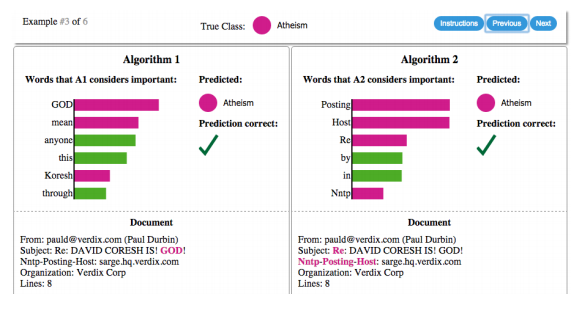
\includegraphics[width=0.9\linewidth]{Images/AtheismExample}
		\caption[LIME-Text-Example]{LIME-Text: predicting "Atheism" for given text }
		\label{fig:atheismexample}
	\end{figure}
	\begin{center}
		Both algorithms predict correct - yet Algorithm 2 has strange reasons.
	\end{center}
\end{frame}

\begin{frame}
	\frametitle{Trusting a Model}
	\begin{center}
		\begin{Large}
			trusting predictions $\neq$ trusting a model
		\end{Large}
	\end{center}
~\newline ~\newline 
	What do we want? 
	\begin{enumerate}
		\item get an \textit{overview} of our Model
		\item compare models in reasonable time
		\item proove correctness \& flaws of a model
		\item improve our models
	\end{enumerate}
\end{frame}

\begin{frame}
	\frametitle{Prooving a Model}
	Several topics which benefit from machine learning, but need special care: 
	\begin{Large}
		\begin{enumerate}
			\item Terrorism-detection
			\item Medical diagnosis \& prescriptions
			\item Fraud-detection
		\end{enumerate}
	\end{Large}

	Noone will buy a model, if you can't prove that it's performing reasonable predictions.
\end{frame}
\begin{frame}
	\frametitle{Improving a Model}
	There are several issues, at which explanations can help you improve your models:
	~\newline
	\begin{Large}
		\begin{enumerate}
			\item Filtering of Features
			\item Find overfitted weighting of features
			\item Find Links in Classification (Similiar Classes and Features)
		\end{enumerate}
	\end{Large}
	~\newline ~\newline
	Gaining insights from explanations can help you improve your model!
\end{frame}